\documentclass[12pt]{article}
\usepackage{ctex}
\usepackage{graphicx}
\usepackage{indentfirst}
\usepackage{amsmath}
\usepackage{float}
\usepackage{amssymb}

\title{第四周作业报告}
\author{佐藤拓未 20300186002}
\date{}

\begin{document}
	\maketitle
	\begin{center}
		\textbf{第一问}
	\end{center}
证明隐式Euler格式是一阶收敛的\\
\\
\noindent \textbf{证明:}考虑系统$\frac{{\rm d}u}{{\rm d}t}=f(t,u)$,$f$关于$u$是L-lipshitz连续,且$\vert\vert u^{''}\vert\vert_{C[0,T]}\le M$\\
联立以下二式

\begin{center}
		\begin{cases}
			u(t_{n+1})&=u(t_n)+\Delta{t}f(t_{n+1},u(t_{n+1}))+R_{n+1}\\
			u_{n+1}&=u_n+\Delta{t}f(t_{n+1},u_{n+1})
		\end{cases}
\end{center}
\noindent 记$e_{n+1}=u(t_{n+1})-u_{n+1}$,则有以下
\begin{align*}
	\vert e_{n+1}\vert&\le\vert e_n\vert + L\Delta{t}\vert e_{n+1}\vert + \vert R_{n+1}\vert\\
	&\le \vert e_n\vert + L\Delta{t}\vert e_{n+1}\vert +  \frac{M\Delta{t}^2}{2}
\end{align*}
那么
$$\vert e_{n+1}\vert \le \frac{1}{1-L\Delta{t}}\vert e_n\vert+\frac{1}{1-L\Delta{t}}\frac{M\Delta{t}^2}{2}$$

\noindent 再考虑如下,当$\Delta{t}$足够小时有$L\Delta{t}\le \frac{1}{2}$时
$$\frac{1}{1-L\Delta{t}}=\frac{1-(L\Delta{t})^2+(L\Delta{t})^2}{1-L\Delta{t}}\le1+L\Delta{t}+\frac{(L\Delta{t})^2}{1-L\Delta{t}}\le 1+ 3L\Delta{t}$$



\noindent 也有$\frac{1}{1-L\Delta{t}}\le2$,从而
\begin{align*}
	\vert e_{n+1}\vert&\le(1+3L\Delta{t})\vert e_n\vert+M\Delta{t}^2\\
	&\le(1+3L\Delta{t})^{n+1}\vert e_0\vert+M(\sum_{k=0}^{n+1}(1+3L\Delta{t})^k)\Delta{t}^2
\end{align*}
考虑$(1+3L\Delta{t})^{n+1}\le e^{3LT}$,其中$T$是有限数,且
\begin{align*}
	\vert e_{n+1}\vert &\le e^{3LT}\vert e_0\vert +M(n+1)e^{3LT}\Delta{t}^2\\
	&\le e^{3LT}\vert e_0\vert + M\frac{(n+1)\Delta{t}}{\Delta{t}}e^{3LT}\Delta{t}^2\\
	&\le e^{3LT}\vert e_0\vert + MTe^{3LT}\Delta{t}
\end{align*}
\noindent 再由$\vert e_0\vert =0$,就可知隐式Euler格式是一阶收敛的。\\

\begin{center}
	\textbf{第二问}
\end{center}
用显式、隐式、改进、修正Euler格式计算$\frac{{\rm d}u}{{\rm d}t}=au$,并用图说明其收敛性(其中$a=-2$,$u_0=1$,$T=1$,$\Delta{t}$任取)\\
\\
\noindent \textbf{解:}设不同格式的迭代初值$u_0=1$
\\利用MATLAB分别建立显式、隐式、改进、修正Euler格式的子程序,并分别利用子程序绘制在步长$\Delta{t}=0.08$下近似解的图像,各近似解以及它们与精确解$u(t)=e^{-2t}$的绝对误差如下所示:
\begin{figure}[H]
	\centering
	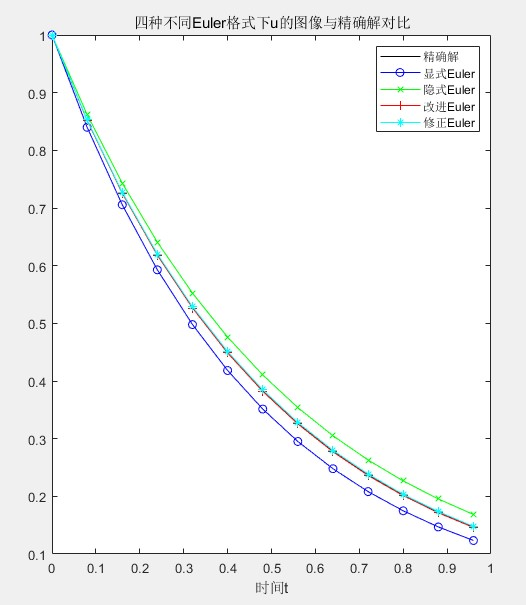
\includegraphics[width=1\textwidth]{1}
	\caption{步长为0.08;横坐标对应了时间t;纵坐标对应不同近似解以及精确解的函数值}
\end{figure}
\begin{figure}[H]
	\centering
	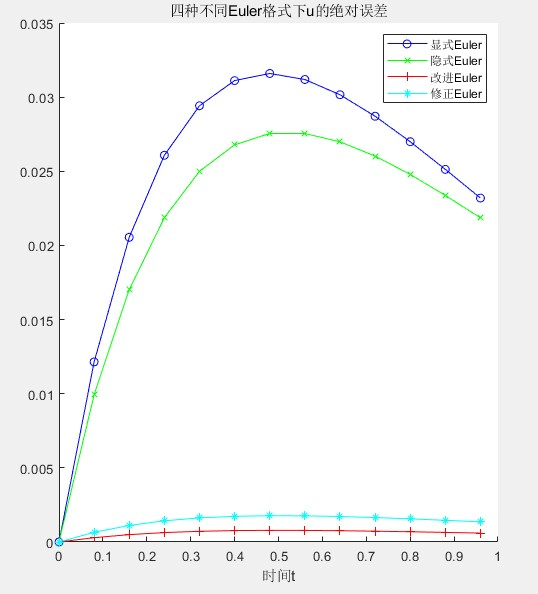
\includegraphics[width=1\textwidth]{2}
	\caption{步长为0.08;横坐标对应了时间t;纵坐标对应不同近似解与精确解的绝对误差}
\end{figure}
从上图可以看出,当步长$\Delta{t}=0.08$时,显式Euler与隐式Euler格式的精度式较差的,它们的最大误差分别达到了$3.16\times10^{-2}$以及$2.75\times10^{-2}$;而改进与修正Euler格式的精度相当且收敛精度较好,它们的绝对误差控制在$1.8\times10^{-3}$以内。\\


\begin{center}
	\textbf{第三问}
\end{center}
给出修正和改进Euler格式的稳定性分析和绝对稳定区间\\
\\
\textbf{解:}
绝对问题区间考虑测试问题$\frac{{\rm d}u}{{\rm d}t}=au$\\
对于改进的Euler格式:$u_{n+1}=u_n+\Delta{t}f_{n+\frac{1}{2}}$,其中$f_{n+\frac{1}{2}}=\frac{f_n+f_{n+1}}{2}$\\
首先考虑其扰动:设现有扰动$\widetilde{u_{n+1}}=\widetilde{u_n}+\frac{\Delta{t}(f(t_n,\widetilde{u_n})+f(t_{n+1},\widetilde{u_{n+1}}))}{2}$,那么由$u_{n+1}=u_n+\frac{a\Delta{t}}{2}(u_n+u_{n+1})$,可知$u_{n+1}=(1+\frac{a\Delta{t}}{1-\frac{a\Delta{t}}{2}})u_n$,也有
\begin{align*}
	{\widetilde{e_{n+1}}}&= u_{n+1}-\widetilde{u_{n+1}}  \\
	&=(1+\frac{a\Delta{t}}{1-\frac{a\Delta{t}}{2}})^{n+1} \widetilde{e_0}=(\frac{1+\frac{a\Delta{t}}{2}}{1-\frac{a\Delta{t}}{2}})^{n+1}\widetilde{e_0}
\end{align*}
考虑改进的Euler格式的绝对稳定区域:由上讨论可知,只需要$$\vert(1+\frac{a\Delta{t}}{1-\frac{a\Delta{t}}{2}})\vert\le1$$
令$z=a\Delta{t}$,就有改进的Euler格式的绝对稳定区域$\{ \vert\frac{2+z}{2-z}\vert \le1 \}$


\noindent 而对于一般的系统$\frac{{\rm d}u}{{\rm d}t}=f(t,u)$,且$f$关于$u$是$L$-lipschitz连续,经计算可知有如下$$\vert \widetilde{e_{n+1}}\vert \le(\frac{1+\frac{L\Delta{t}}{2}}{1-\frac{L\Delta{t}}{2}})^{n+1}\vert \widetilde{e_0}\vert$$
不妨就令$L=\vert a\vert$:当$\Delta{t}$足够小时,有$\frac{\vert a\vert\Delta{t}}{1-\frac{\vert a\vert\Delta{t}}{2}}\le2\vert a \vert\Delta{t}$,且$(1+2\vert a\vert\Delta{t})^{n+1}=(1+2\vert a\vert\Delta{t})^{(n+1)\frac{1}{2\vert a\vert\Delta{t}}2\vert a\vert\Delta{t}}\le e^{2\vert a\vert\Delta{t}(n+1)}$,从而$$\vert \widetilde{e_{n+1}}\vert\le e^{2\vert a\vert T}\vert \widetilde{e_0}\vert$$其中$T$有限,从而可知改进的Euler格式是稳定的\\

\\


\noindent 对于修正的Euler格式:$u_{n+1}=u_n+\Delta{t}f_{n+\frac{1}{2}}$,其中$f_{n+\frac{1}{2}}=f(t_{n+\frac{1}{2}},u_n+\frac{\Delta{t}}{2}f_n)$\\
可知测试问题中,$u_{n+1}=u_n+a\Delta{t}(u_n+\frac{\Delta{t}}{2}f_n)$,进一步可知
\begin{align*}
	\widetilde{e_{n+1}}&=\widetilde{e_{n}}+ a \Delta{t}[(u_n-\widetilde{u_n})+\frac{\Delta{t}}{2}(f_n-\widetilde{f_n})]\\
	&=(1+ a\Delta{t}+\frac{( a\Delta{t})^2}{2})\widetilde{e_{n}}
\end{align*}
\noindent 令$z= a \Delta{t}$,可知修正的Euler格式的绝对稳定区域$\{\vert 1+z+ \frac{z^2}{2} \vert \le1\}$\\
一般地,可知当$f$是关于$u$为$\vert a\vert$-lipschitz连续时
\begin{align*}
	\vert\widetilde{e_{n+1}}\vert&\le \vert \widetilde{e_{n}}\vert + \vert a\vert \Delta{t}\vert \widetilde{e_{n}}\vert +\frac{\vert a\vert \Delta{t}^2}{2}\vert f_n-\widetilde{f_n}\vert\\
	&\le(1+\vert a\vert\Delta{t} + \frac{(\vert a \Delta{t}\vert^2)}{2})^{n+1}\vert \widetilde{e_0}\vert
\end{align*}
当$\Delta{t}$足够小时,$\frac{(\vert a \Delta{t}\vert^2)}{2}\le \vert a\vert\Delta{t} $,从而有$\vert\widetilde{e_{n+1}}\vert\le (1+2\vert a\vert \Delta{t})^{n+1}\vert \widetilde{e_0}\vert$,那么由上面的讨论可得$\vert\widetilde{e_{n+1}}\vert\le e^{2\vert a\vert T}\vert \widetilde{ e_0}\vert$,知修正的Euler格式是稳定的\\


\begin{center}
	\textbf{第四问}
\end{center}
用Taylor级数法,$q=1,2,3$,计算:$$\frac{{\rm d}u}{{\rm d}t}=u-u^2$$画图说明精度\\
\\
\noindent \textbf{解:}$u(t)=\frac{1}{(\frac{1}{u_0}-1)e^{-t}+1}$,其中$u_0\ge0$,以及$\phi(t,u(t);\Delta{t})=\sum_{j=1}^{q}\frac{\Delta{t}^{j-1}}{j!}\frac{{\rm d}^{j-1}f(t,u(t))}{{\rm d} t^{j-1}}$\\
当$q=1$时,$u_{n+1}=u_n+\Delta{t}\phi(t_n,u_n;\Delta{t})=u_n+\Delta{t}f(t_n,u_n)=u_n+\Delta{t}u_n-\Delta{t}u_n^2$\\
当$q=2$时,$u_{n+1}=u_n+\Delta{t}f(t_n,u_n)+\frac{\Delta{t}^2}{2}[f^{'}_t(t_n,u_n)+f^{'}_u(t_n,u_n)f(t_n,u_n)]$\\$=u_n+\Delta{t}u_n-\Delta{t}u_n^2+\frac{\Delta^2}{2}[(1-2u_n)(u_n-u_n^2)]$\\
当$q=3$时,$u_{n+1}=u_n+\Delta{t}u_n-\Delta{t}u_n^2+\frac{\Delta^2}{2}[(1-2u_n)(u_n-u_n^2)]+\frac{\Delta{t}^3}{6}[-2(u_n-u_n^2)^2+(1-2u_n)^2(u_n-u_n^2)]$\\
事实上,$q=2,3$时也可以看作是显式Euler格式,将$\phi(t_n,u_n;\Delta{t})$代入第二问中的子程序即可得出对应的近似解。\\
当$u_0=0.5,t_0=0,T=1,\Delta{t}=0.08$的图像如下图所示:
\begin{figure}[H]
	\centering
	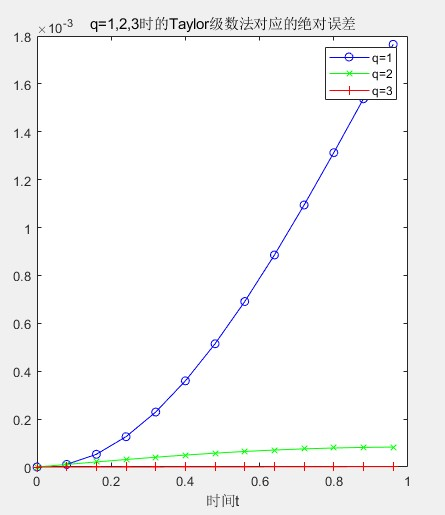
\includegraphics[width=1\textwidth]{3}
	\caption{初值为0.5;步长为0.08;横坐标对应了时间t;纵坐标对应不同近似解与精确解的绝对误差}
\end{figure}
\noindent 当$u_0=0.5,t_0=0,T=1,\Delta{t}=0.08$时,$q=1$的收敛精度控制在$1.8\times10^{-3}$以内;$q=2,3$的收敛精度均控制在$8.4\times10^{-5}$以内。可知此情形下,$q=2,3$的收敛精度要优越得多。\\
当$u_0=1.5,t_0=0,T=1,\Delta{t}=0.08$时的图像如下:
\begin{figure}[H]
	\centering
	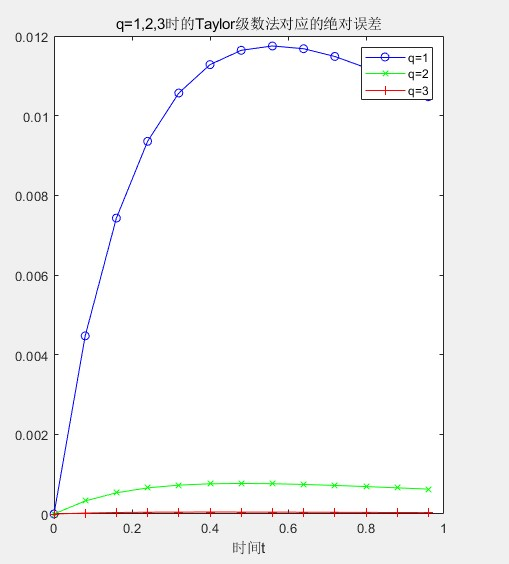
\includegraphics[width=1\textwidth]{4}
	\caption{初值为1.5;步长为0.08;横坐标对应了时间t;纵坐标对应不同近似解与精确解的绝对误差}
\end{figure}
\noindent
当$u_0=1.5,t_0=0,T=1,\Delta{t}=0.08$时,$q=1$的收敛精度控制在$1.2\times10^{-3}$以内;$q=2,3$的收敛精度均控制在$7.7\times10^{-4}$以内。\\
总之,随着$q$越来越高,Taylor级数法的精度会越来越高。
\end{document}